\section{API végpontok részletes bemutatása}

A backend végpontjait a Postman alkalmazás segítségével követtük nyomon, amely lehetővé teszi HTTP-alapú API-k vizuális kezelését, tesztelését és dokumentálását. A fejlesztés során a Postmant nemcsak hibakeresésre, hanem a végpontok működésének gyors ellenőrzésére és az API tervezés vizualizálására is használtuk. Lehetőséget ad az egyes kérések testreszabására (pl. fejlécek, paraméterek, autentikáció), valamint az API válaszainak könnyű értelmezésére.

\begin{itemize}
    \item \textbf{GET /v1/get\_stations\_by\_city} – Ez az API végpont lehetővé teszi, hogy egy adott városhoz tartozó állomásokat kérjünk le. Ezen végpont segítségével a felhasználók gyorsan megtalálhatják azokat az állomásokat, amelyek egy meghatározott városhoz tartoznak. A kérés paraméterei tartalmazzák a város nevét, és a válasz egy listát ad vissza az állomásokró, amint azt a \ref{fig:postman_get_stations_by_city} ábra is mutatja.
    \begin{figure}[H]
        \centering
        
\includegraphics[width=0.8\textwidth]{figures/postman_request_get_stations_by_city.png}
        \caption{A \texttt{GET /v1/get\_stations\_by\_city} végpont kérésének paraméterei és válasza}
        \label{fig:postman_get_stations_by_city}
    \end{figure}

    \item \textbf{GET /v1/get\_available\_tickets} – A \ref{fig:postman_get_available_tickets} ábrán is látható módon ez végpont lehetővé teszi az elérhető jegyek lekérdezését egy adott kiindulási és célállomás között. A kérés paraméterei a kiindulási és célállomás, valamint egy opcionális időpont. A megállók is opcionálisak, a csak a város megadása esetén minden megállóhoz láthatjuk a jegyeket. A válasz tartalmazza az elérhető jegyek listáját, és ezek árai.
    \begin{figure}[H]
        \centering
        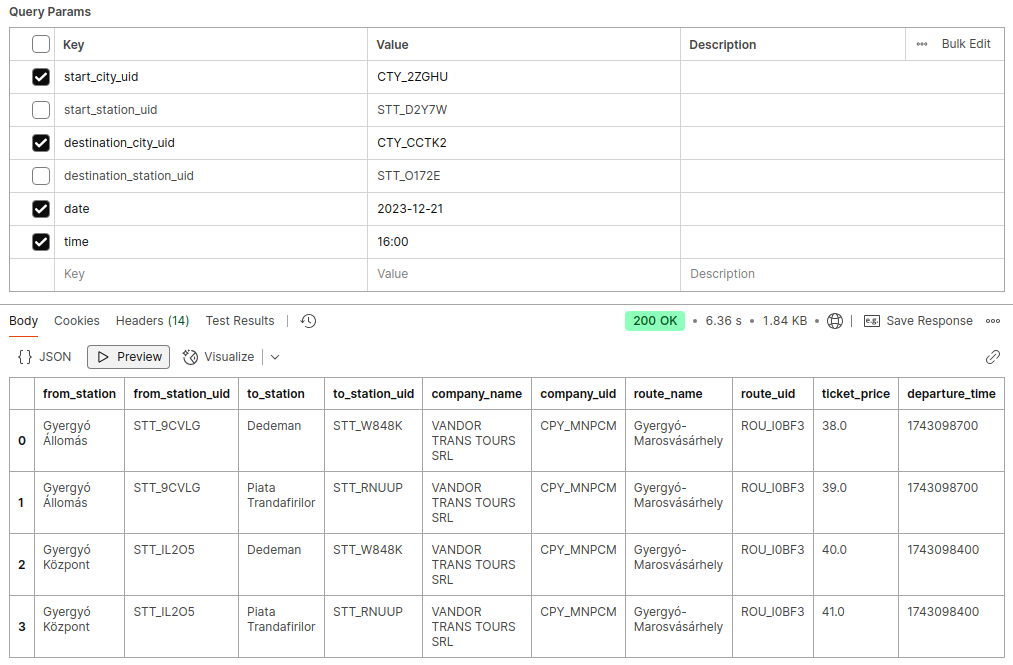
\includegraphics[width=0.8\textwidth]{figures/postman_request_get_available_tickets.png}
        \caption{A \texttt{GET /v1/get\_available\_tickets} végpont kérésének paraméterei és válasza}
        \label{fig:postman_get_available_tickets}
    \end{figure}

    \item \textbf{GET /v1/get\_bus\_locations\_by\_route} – Ezen API végpont segítségével lekérhetjük a buszok aktuális helyzetét egy adott járatra vonatkozóan. A kérés tartalmazza a járat azonosítóját, és a válasz egy koordinátákkal mutatja a buszok aktuális pozícióit, amint azt a \ref{fig:postman_get_bus_locations} ábra is mutatja.
    \begin{figure}[H]
        \centering
        
\includegraphics[width=0.8\textwidth]{figures/postman_request_get_bus_locations.png}
        \caption{A \texttt{GET /v1/get\_bus\_locations\_by\_route} végpont kérésének paraméterei és válasza}
        \label{fig:postman_get_bus_locations}
    \end{figure}

    \item \textbf{GET /v1/tickets\_of\_user} – Az aktuális felhasználó jegyeinek lekérésére szolgáló végpont. A kérés nem tartalmaz paramétereket, mivel az aktuális felhasználó jegyeit kérdezi le. A válaszban szereplő jegyek információi tartalmazzák a jegyek típusát, érvényességüket és egyéb fontos adatokat, a \ref{fig:postman_get_tickets_of_user} ábrán látható módon.
    \begin{figure}[H]
        \centering
        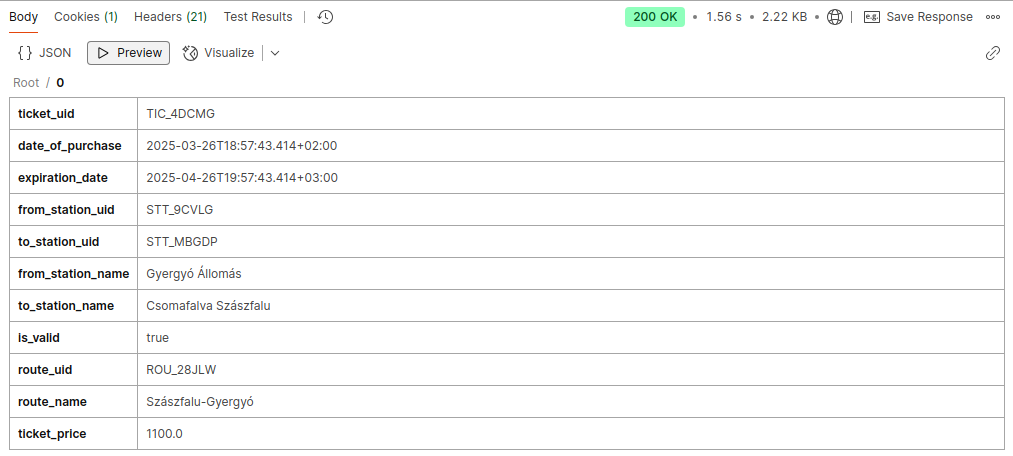
\includegraphics[width=0.8\textwidth]{figures/postman_request_get_tickets_of_user.png}
        \caption{A \texttt{GET /v1/tickets\_of\_user} végpont kérésének paraméterei és válasza}
        \label{fig:postman_get_tickets_of_user}
    \end{figure}

    \item \textbf{POST /v1/admin/add\_station\_to\_route} – Ez az adminisztrátorok számára elérhető végpont lehetővé teszi egy állomás hozzárendelését egy adott útvonalhoz. A kérés tartalmazza az útvonal és az állomás azonosítóját, és a válasz megerősíti a sikeres műveletet, amint a \ref{fig:postman_add_station_to_route} ábrán is látható.
    \begin{figure}[H]
        \centering
        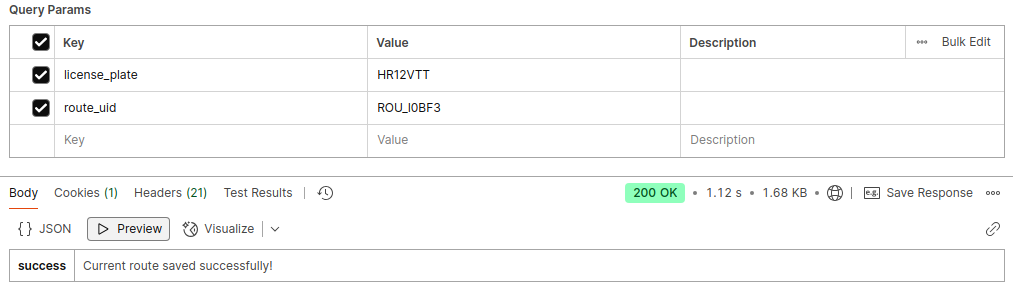
\includegraphics[width=0.8\textwidth]{figures/postman_request_add_station_to_route.png}
        \caption{A \texttt{POST /v1/admin/add\_station\_to\_route} végpont kérésének paraméterei és válasza}
        \label{fig:postman_add_station_to_route}
    \end{figure}
\end{itemize}

\section{Adatbázis kapcsolat}

Az API végpontjai a PostgreSQL adatbázissal kommunikálnak. Az adatbázis tranzakciókat az ActiveRecord ORM segítségével kezeljük, amely lehetővé teszi az adatok egyszerű és hatékony lekérését, beszúrását és frissítését.

\subsection{Adatbázis táblák}
A PostgreSQL adatbázisunk a következő táblákból áll:
\begin{itemize}
    \item \textbf{Companies}: Azon cégek adatai, akikkel szerződést kötött a Bus4U.
    \item \textbf{Admins}: Különböző cégekhez tartozó adminisztrátorok adatai. Szerepük lehet “boss” vagy “driver”.
    \item \textbf{Buses}: A cégekhez tartozó autóbuszok adatai.
    \item \textbf{Routes}: A cégek saját útvonalai.
    \item \textbf{Stations}: A rendszerben található buszmegállók összessége.
    \item \textbf{Route\_stations}: Egy cég adott útvonalán keresztülhaladó megállók.
    \item \textbf{Timetables}: Egy útvonal megállójának indulási időpontjai és ára nap szerinti felosztásban.
    \item \textbf{Cities}: Az összes város, amelyen áthaladnak útvonalak.
    \item \textbf{Users}: A Bus4U felhasználói a fontosabb adataikkal.
    \item \textbf{Email\_verifications}: Az adott email címekhez tartozó regisztrációkor felhasználandó kódok.
    \item \textbf{Tickets}: A felhasználókhoz tartozó jegyek.
    \item \textbf{Payments}: Stripe fizetések eltárolása.
\end{itemize}

A táblák közötti kapcsolatokat a \ref{fig:database-diagram} ábra szemlélteti.

\begin{figure}[H]
    \centering
    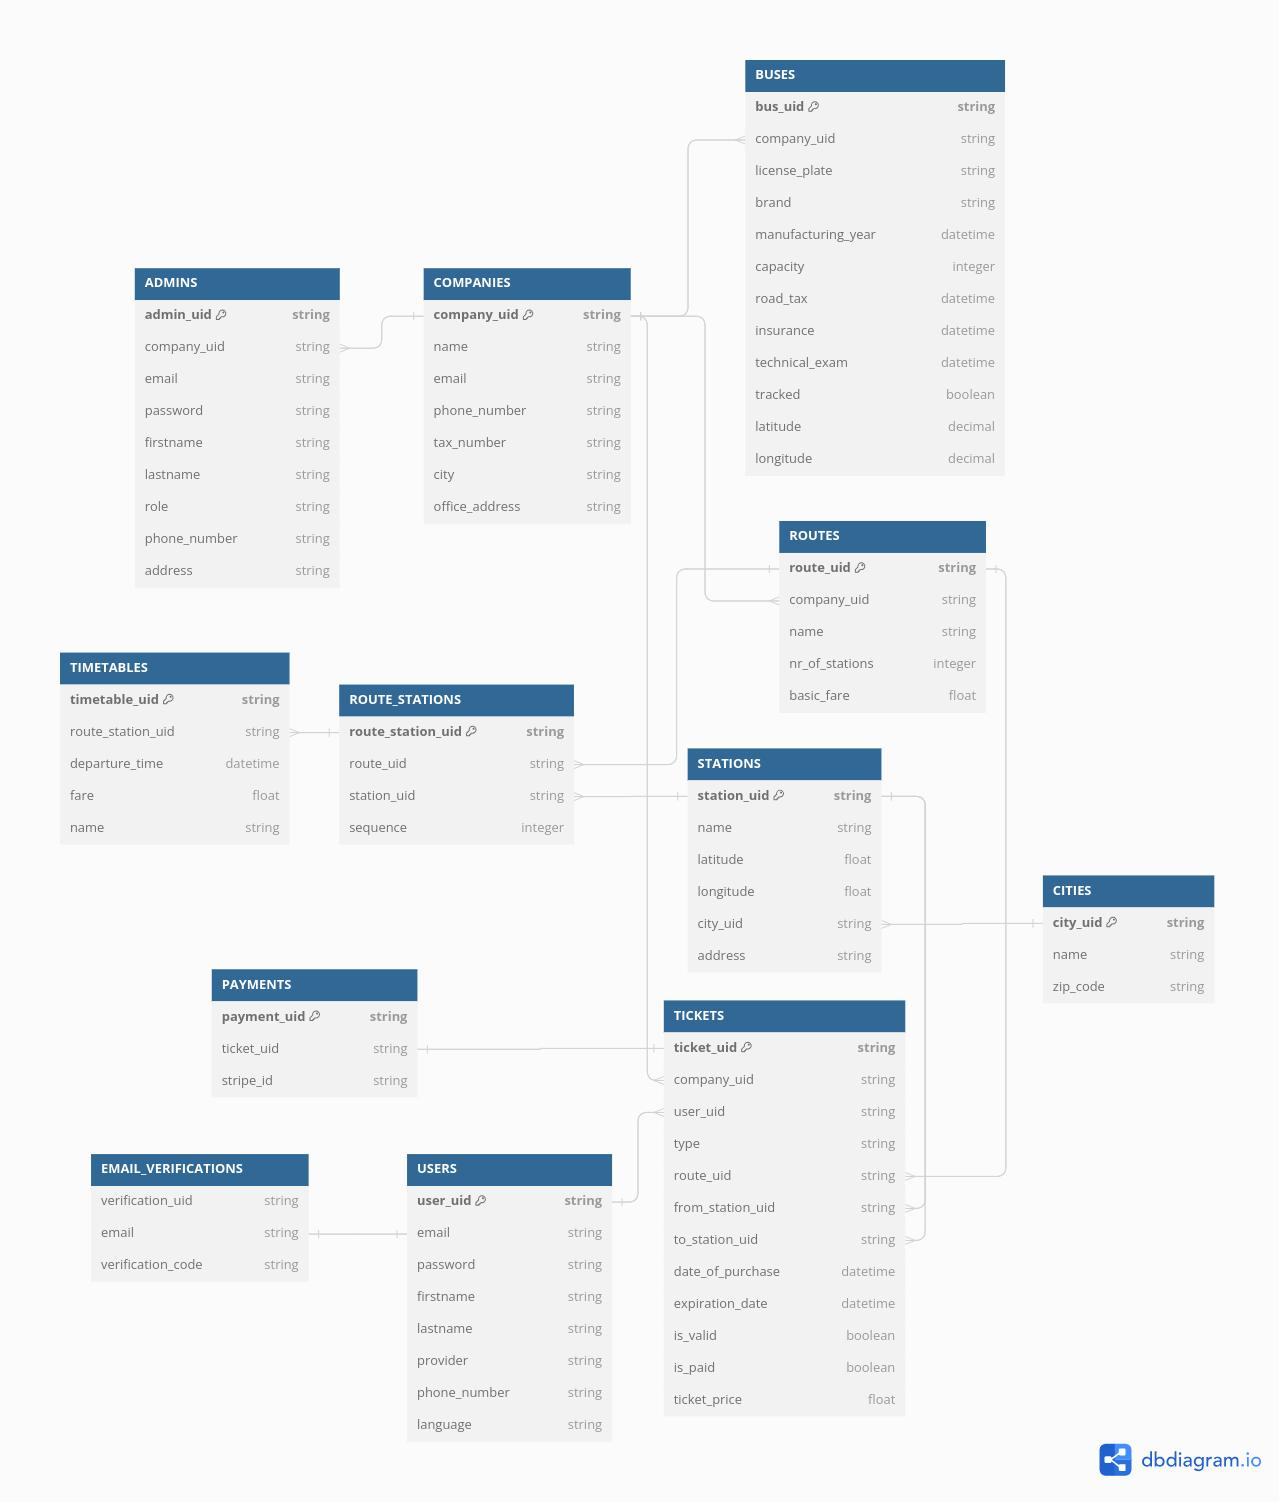
\includegraphics[width=\textwidth]{figures/database.jpg}
    \caption{Az rendszer adatbázisdiagramja}
    \label{fig:database-diagram}
  \end{figure}

  \subsection{Objektum-relációs leképzés (ORM)}

  A backend API adatbázis-kezelése a Ruby on Rails keretrendszer beépített ActiveRecord objektum-relációs leképzőjével (ORM) történik. Az ORM lehetővé teszi az alkalmazás számára, hogy közvetlenül Ruby osztályok és objektumok formájában kezelje az adatbázis tábláit, így egyszerűsítve az adatbázis-műveleteket és csökkentve a fejlesztési időt.
  
  Az ActiveRecord fő előnyei közé tartozik:
  \begin{itemize}
      \item \textbf{Egyszerű adatlekérdezés:} A komplex SQL utasítások helyett Ruby nyelven írhatók a lekérdezések.
      \item \textbf{Adatkapcsolatok automatikus kezelése:} Egyértelművé teszi az adatok közötti kapcsolatokat (például \texttt{belongs\_to}, \texttt{has\_many}, \texttt{has\_one}).
      \item \textbf{Validációk és tranzakciók egyszerű kezelése:} Adatvalidáció, tranzakciókezelés és hibaüzenetek egyszerű integrációja az üzleti logikába.
      \item \textbf{Migrációk támogatása:} Könnyű adatbázis-struktúra módosítás a migrációs fájlokon keresztül.
  \end{itemize}
  
  Az ActiveRecord használata jelentősen egyszerűsíti a fejlesztési folyamatot, lehetővé téve, hogy a fejlesztők elsősorban az üzleti logikára összpontosítsanak, miközben a rendszer hatékonyan és biztonságosan kommunikál a PostgreSQL adatbázissal.
  